\documentclass[11pt]{article}
\usepackage[textwidth=18.0cm, textheight=23.0cm, top=2.0cm]{geometry}
\usepackage{pst-all}
\usepackage{amssymb}
\usepackage{tikz}
\usepackage{underscore}\begin{document}
\pagestyle{empty}


ClassName: \underline{\textbf{Class_03.2bp-11}}
\par
BinSize: \underline{\textbf{40 × 40}}
\par
ReduceSize: \underline{\textbf{40 × 40}}
\par
TypeNum: \underline{\textbf{40}}
\par
Num: \underline{\textbf{40}}
\par
OutS: \underline{\textbf{12800}}
\par
InS: \underline{\textbf{11400}}
\par
Rate: \underline{\textbf{0.891}}
\par
UB: \underline{\textbf{8}}
\par
LB0: \underline{\textbf{8}}
\par
LB: \underline{\textbf{8}}
\par
LBWithCut: \underline{\textbf{8}}
\par
NodeCut: \underline{\textbf{0}}
\par
ExtendedNodeCnt: \underline{\textbf{1}}
\par
GenNodeCnt: \underline{\textbf{1}}
\par
PrimalNode: \underline{\textbf{0}}
\par
ColumnCount: \underline{\textbf{8}}
\par
TotalCutCount: \underline{\textbf{0}}
\par
RootCutCount: \underline{\textbf{0}}
\par
LPSolverCnt: \underline{\textbf{1}}
\par
PricingSolverCnt: \underline{\textbf{0}}
\par
BranchAndBoundNum: \underline{\textbf{1}}
\par
isOpt: \underline{\textbf{true}}
\par
TimeOnInitSolution: \underline{\textbf{600.000 s}}
\par
TimeOnPrimal: \underline{\textbf{0.000 s}}
\par
TimeOnPricing: \underline{\textbf{0.000 s}}
\par
TimeOnRmp: \underline{\textbf{0.063 s}}
\par
TotalTime: \underline{\textbf{600.375 s}}
\par
\newpage


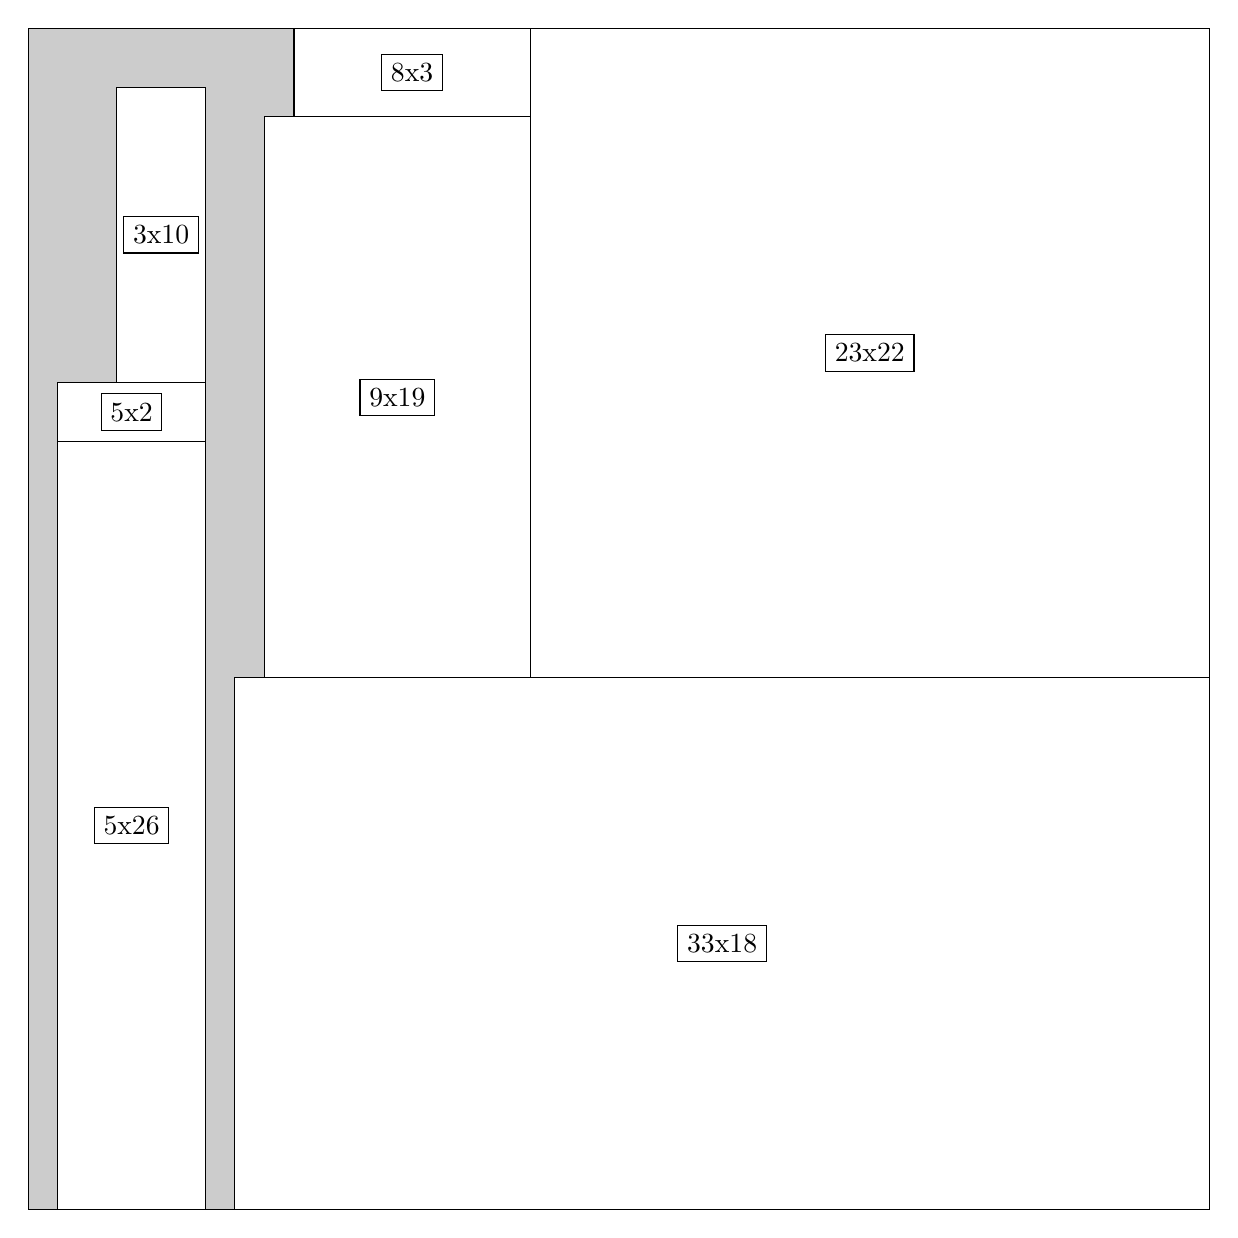
\begin{tikzpicture}[shorten >=1pt,scale=1.0,every node/.style={scale=1.0},->]
\tikzstyle{vertex}=[circle,fill=black!25,minimum size=14pt,inner sep=0pt]
\filldraw[fill=gray!40!white, draw=black] (0,0) rectangle (15.0,15.0);
\foreach \name/\x/\y/\w/\h in {33x18/2.625/0.0/12.375/6.75,23x22/6.375/6.75/8.625/8.25,9x19/3.0/6.75/3.375/7.125,8x3/3.375/13.875/3.0/1.125,5x26/0.375/0.0/1.875/9.75,5x2/0.375/9.75/1.875/0.75,3x10/1.125/10.5/1.125/3.75}
\filldraw[fill=white!40!white, draw=black] (\x,\y) rectangle node[draw] (\name) {\name} ++(\w,\h);
\end{tikzpicture}


w =33 , h =18 , x =7 , y =0 , v =594
\par
w =23 , h =22 , x =17 , y =18 , v =506
\par
w =9 , h =19 , x =8 , y =18 , v =171
\par
w =8 , h =3 , x =9 , y =37 , v =24
\par
w =5 , h =26 , x =1 , y =0 , v =130
\par
w =5 , h =2 , x =1 , y =26 , v =10
\par
w =3 , h =10 , x =3 , y =28 , v =30
\par
\newpage


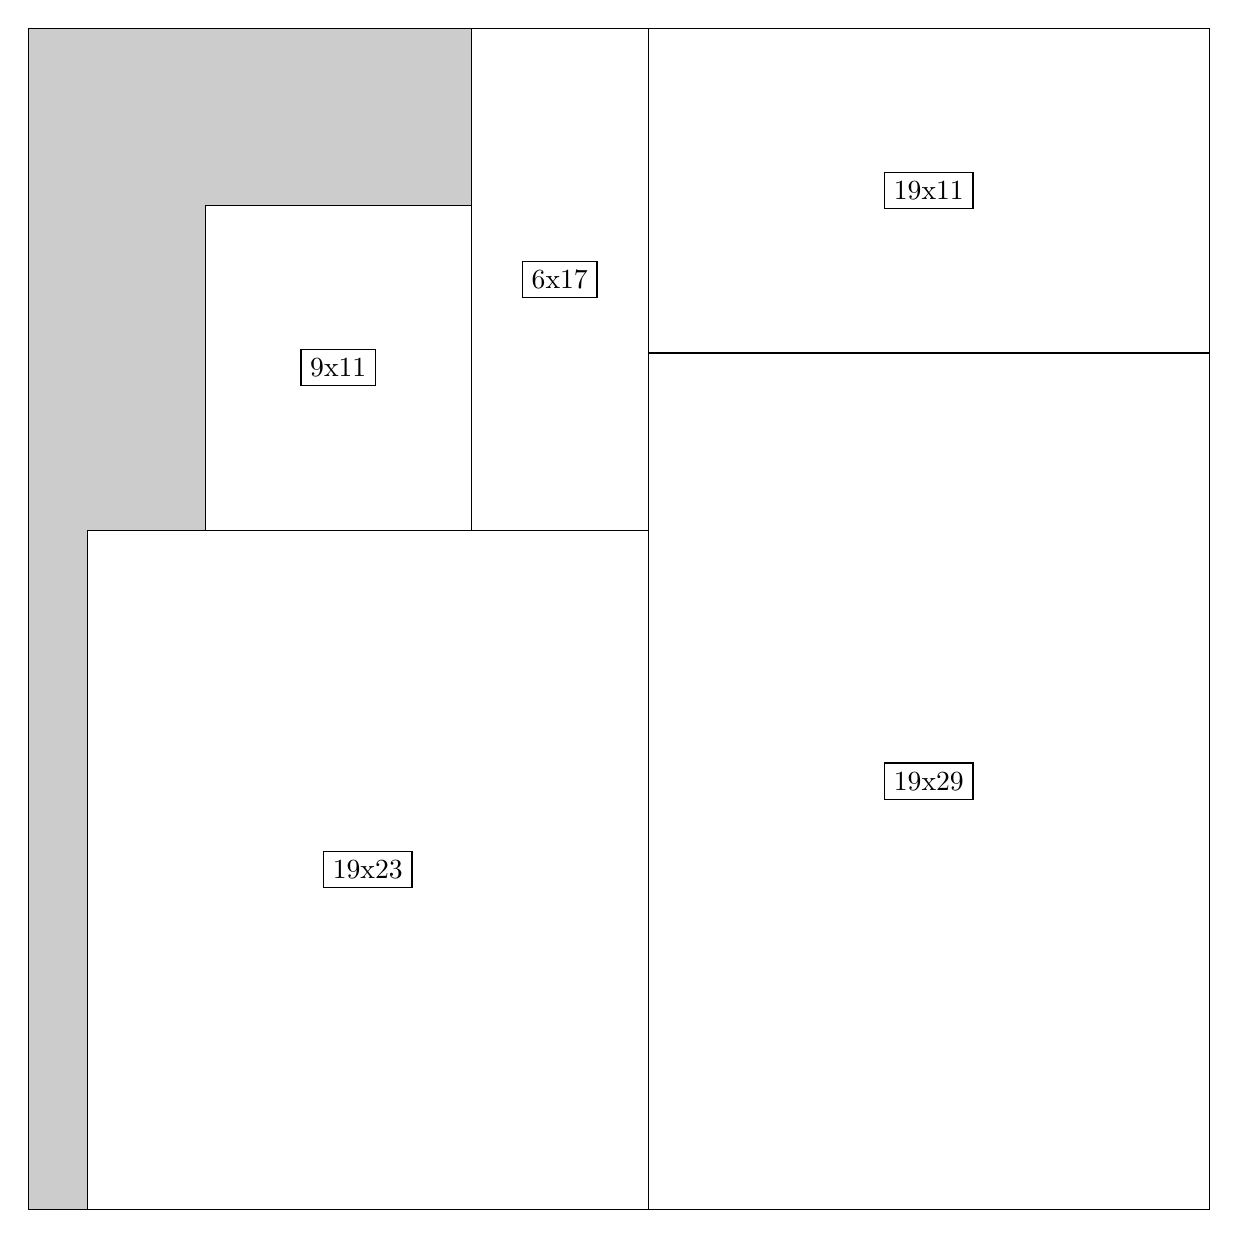
\begin{tikzpicture}[shorten >=1pt,scale=1.0,every node/.style={scale=1.0},->]
\tikzstyle{vertex}=[circle,fill=black!25,minimum size=14pt,inner sep=0pt]
\filldraw[fill=gray!40!white, draw=black] (0,0) rectangle (15.0,15.0);
\foreach \name/\x/\y/\w/\h in {19x29/7.875/0.0/7.125/10.875,19x11/7.875/10.875/7.125/4.125,19x23/0.75/0.0/7.125/8.625,6x17/5.625/8.625/2.25/6.375,9x11/2.25/8.625/3.375/4.125}
\filldraw[fill=white!40!white, draw=black] (\x,\y) rectangle node[draw] (\name) {\name} ++(\w,\h);
\end{tikzpicture}


w =19 , h =29 , x =21 , y =0 , v =551
\par
w =19 , h =11 , x =21 , y =29 , v =209
\par
w =19 , h =23 , x =2 , y =0 , v =437
\par
w =6 , h =17 , x =15 , y =23 , v =102
\par
w =9 , h =11 , x =6 , y =23 , v =99
\par
\newpage


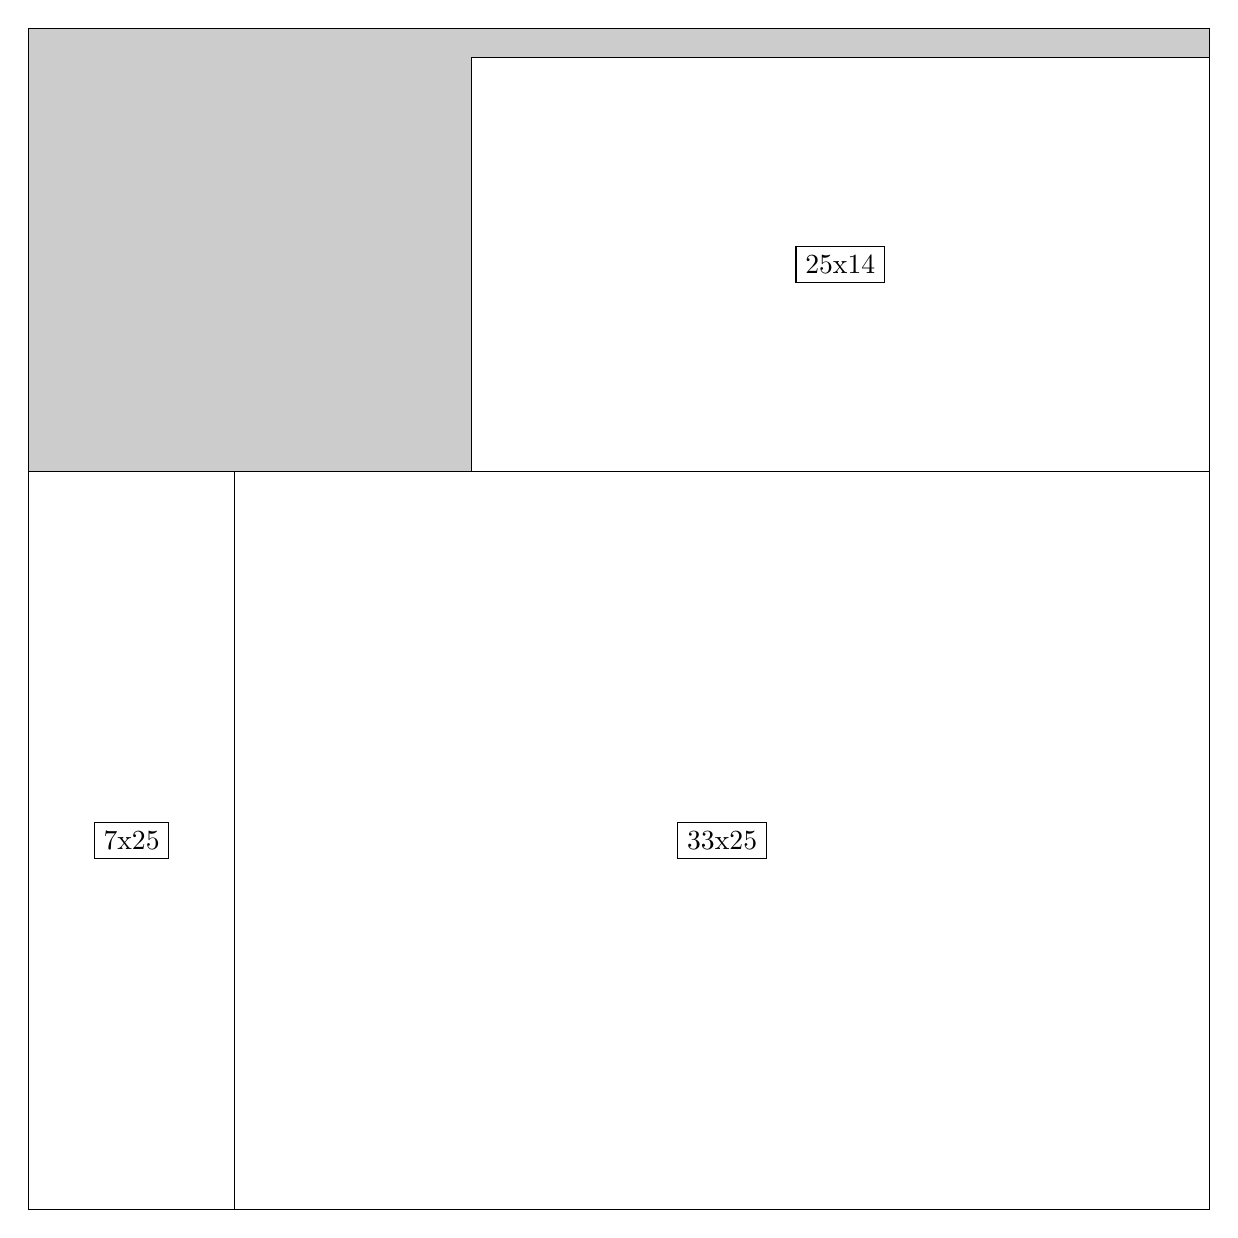
\begin{tikzpicture}[shorten >=1pt,scale=1.0,every node/.style={scale=1.0},->]
\tikzstyle{vertex}=[circle,fill=black!25,minimum size=14pt,inner sep=0pt]
\filldraw[fill=gray!40!white, draw=black] (0,0) rectangle (15.0,15.0);
\foreach \name/\x/\y/\w/\h in {33x25/2.625/0.0/12.375/9.375,25x14/5.625/9.375/9.375/5.25,7x25/0.0/0.0/2.625/9.375}
\filldraw[fill=white!40!white, draw=black] (\x,\y) rectangle node[draw] (\name) {\name} ++(\w,\h);
\end{tikzpicture}


w =33 , h =25 , x =7 , y =0 , v =825
\par
w =25 , h =14 , x =15 , y =25 , v =350
\par
w =7 , h =25 , x =0 , y =0 , v =175
\par
\newpage


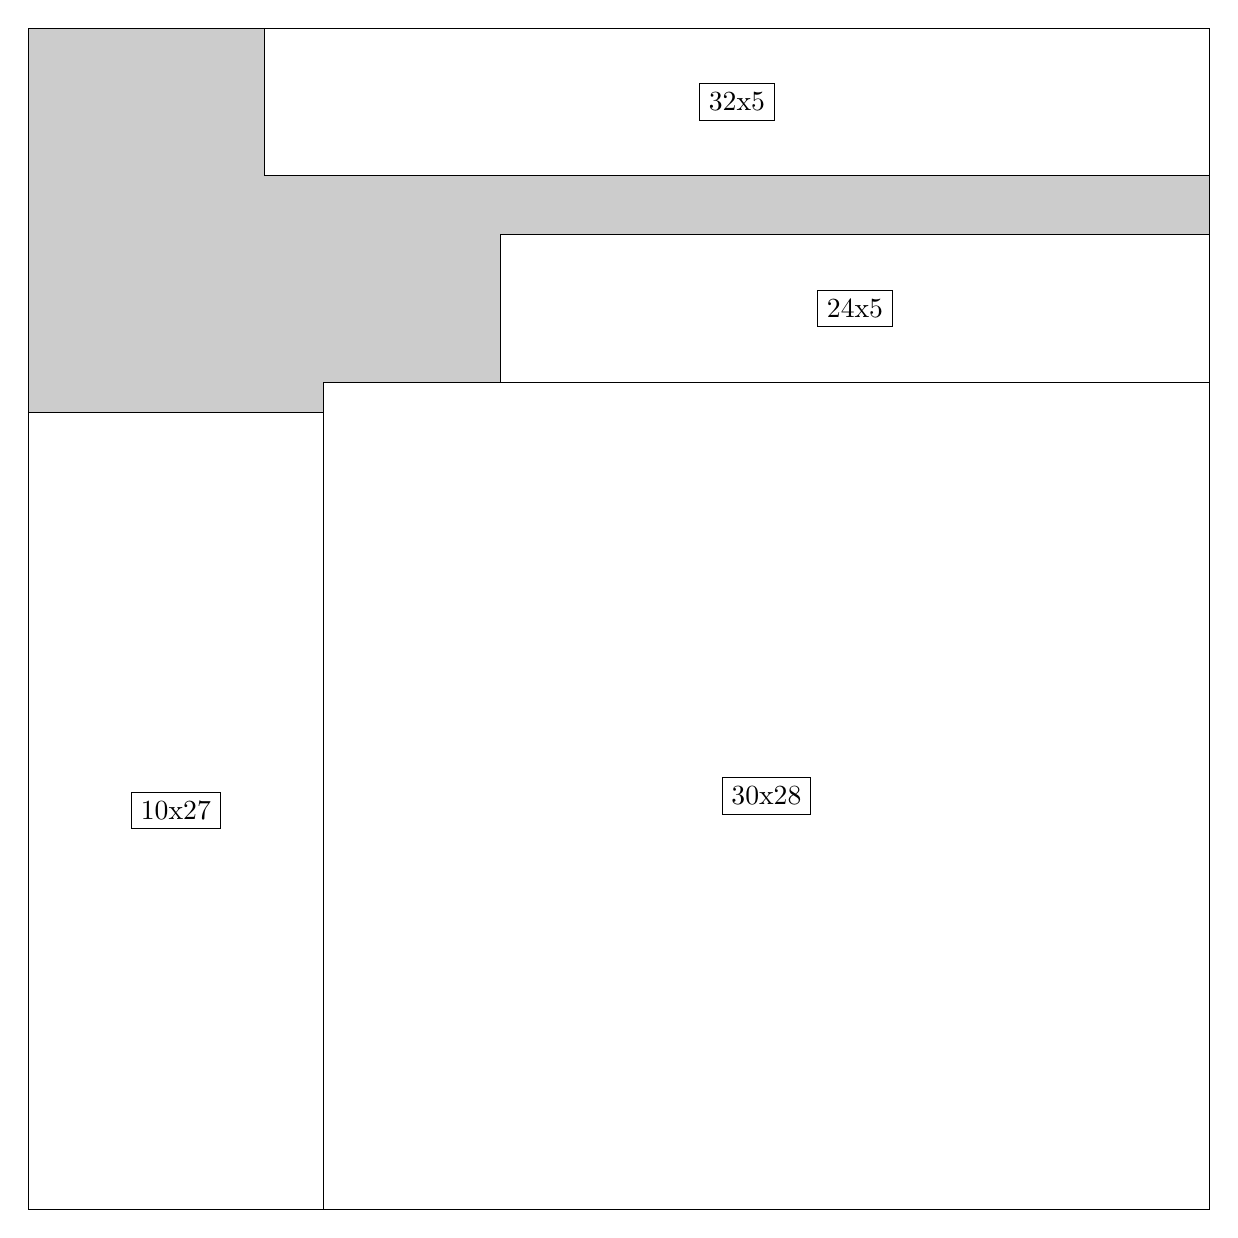
\begin{tikzpicture}[shorten >=1pt,scale=1.0,every node/.style={scale=1.0},->]
\tikzstyle{vertex}=[circle,fill=black!25,minimum size=14pt,inner sep=0pt]
\filldraw[fill=gray!40!white, draw=black] (0,0) rectangle (15.0,15.0);
\foreach \name/\x/\y/\w/\h in {30x28/3.75/0.0/11.25/10.5,24x5/6.0/10.5/9.0/1.875,10x27/0.0/0.0/3.75/10.125,32x5/3.0/13.125/12.0/1.875}
\filldraw[fill=white!40!white, draw=black] (\x,\y) rectangle node[draw] (\name) {\name} ++(\w,\h);
\end{tikzpicture}


w =30 , h =28 , x =10 , y =0 , v =840
\par
w =24 , h =5 , x =16 , y =28 , v =120
\par
w =10 , h =27 , x =0 , y =0 , v =270
\par
w =32 , h =5 , x =8 , y =35 , v =160
\par
\newpage


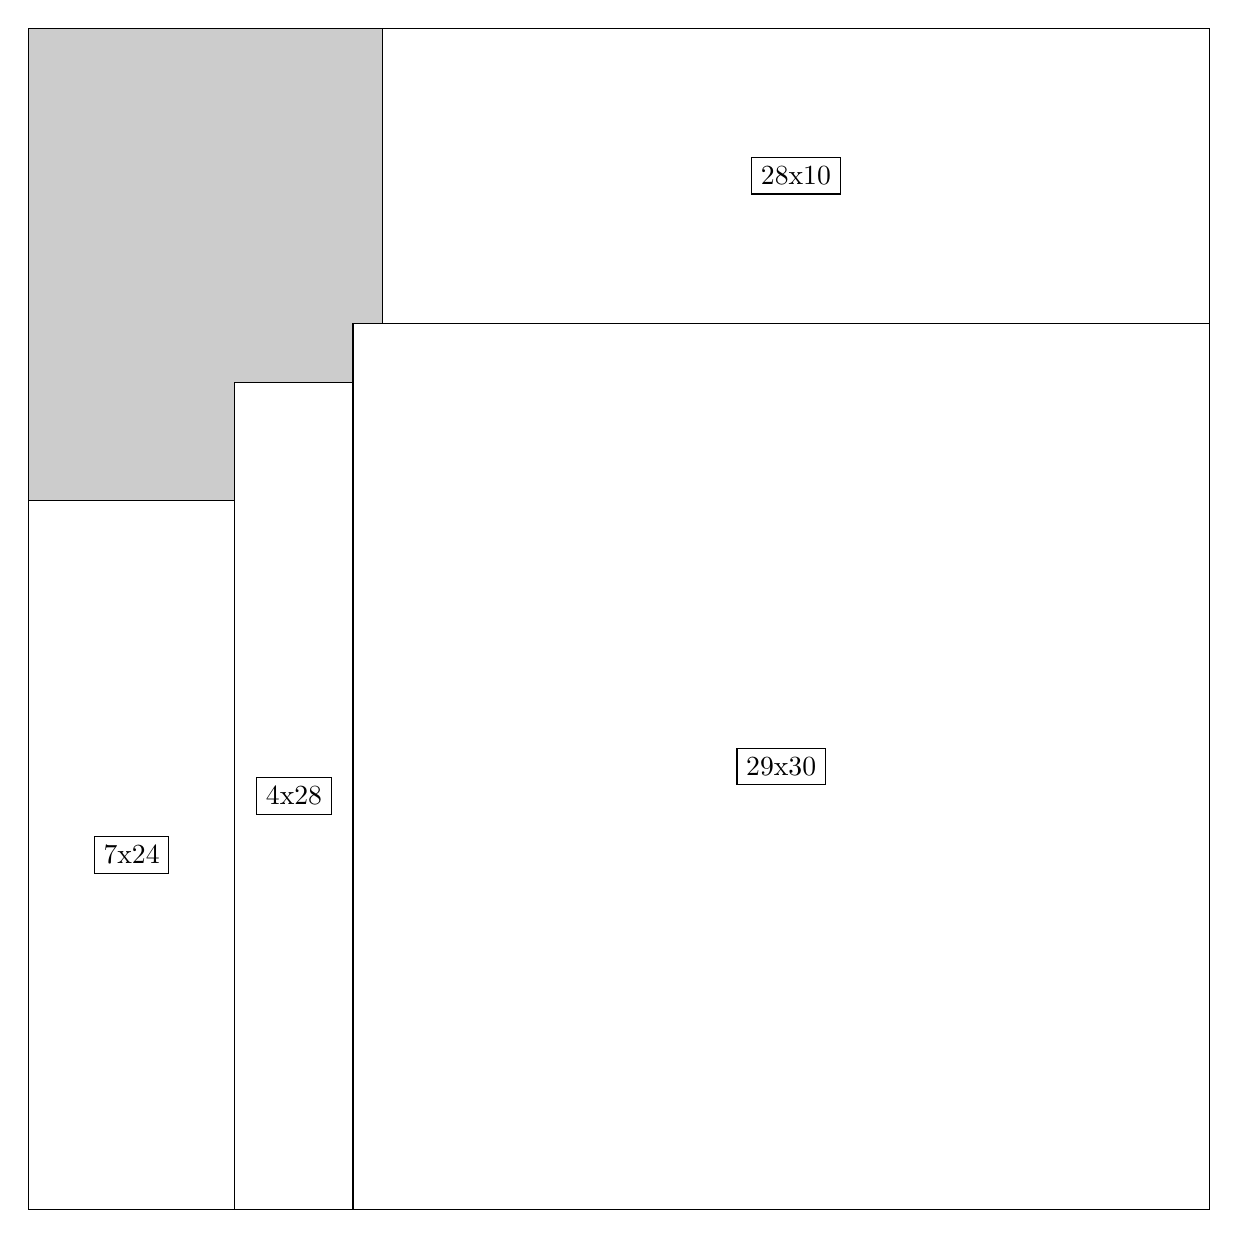
\begin{tikzpicture}[shorten >=1pt,scale=1.0,every node/.style={scale=1.0},->]
\tikzstyle{vertex}=[circle,fill=black!25,minimum size=14pt,inner sep=0pt]
\filldraw[fill=gray!40!white, draw=black] (0,0) rectangle (15.0,15.0);
\foreach \name/\x/\y/\w/\h in {29x30/4.125/0.0/10.875/11.25,4x28/2.625/0.0/1.5/10.5,7x24/0.0/0.0/2.625/9.0,28x10/4.5/11.25/10.5/3.75}
\filldraw[fill=white!40!white, draw=black] (\x,\y) rectangle node[draw] (\name) {\name} ++(\w,\h);
\end{tikzpicture}


w =29 , h =30 , x =11 , y =0 , v =870
\par
w =4 , h =28 , x =7 , y =0 , v =112
\par
w =7 , h =24 , x =0 , y =0 , v =168
\par
w =28 , h =10 , x =12 , y =30 , v =280
\par
\newpage


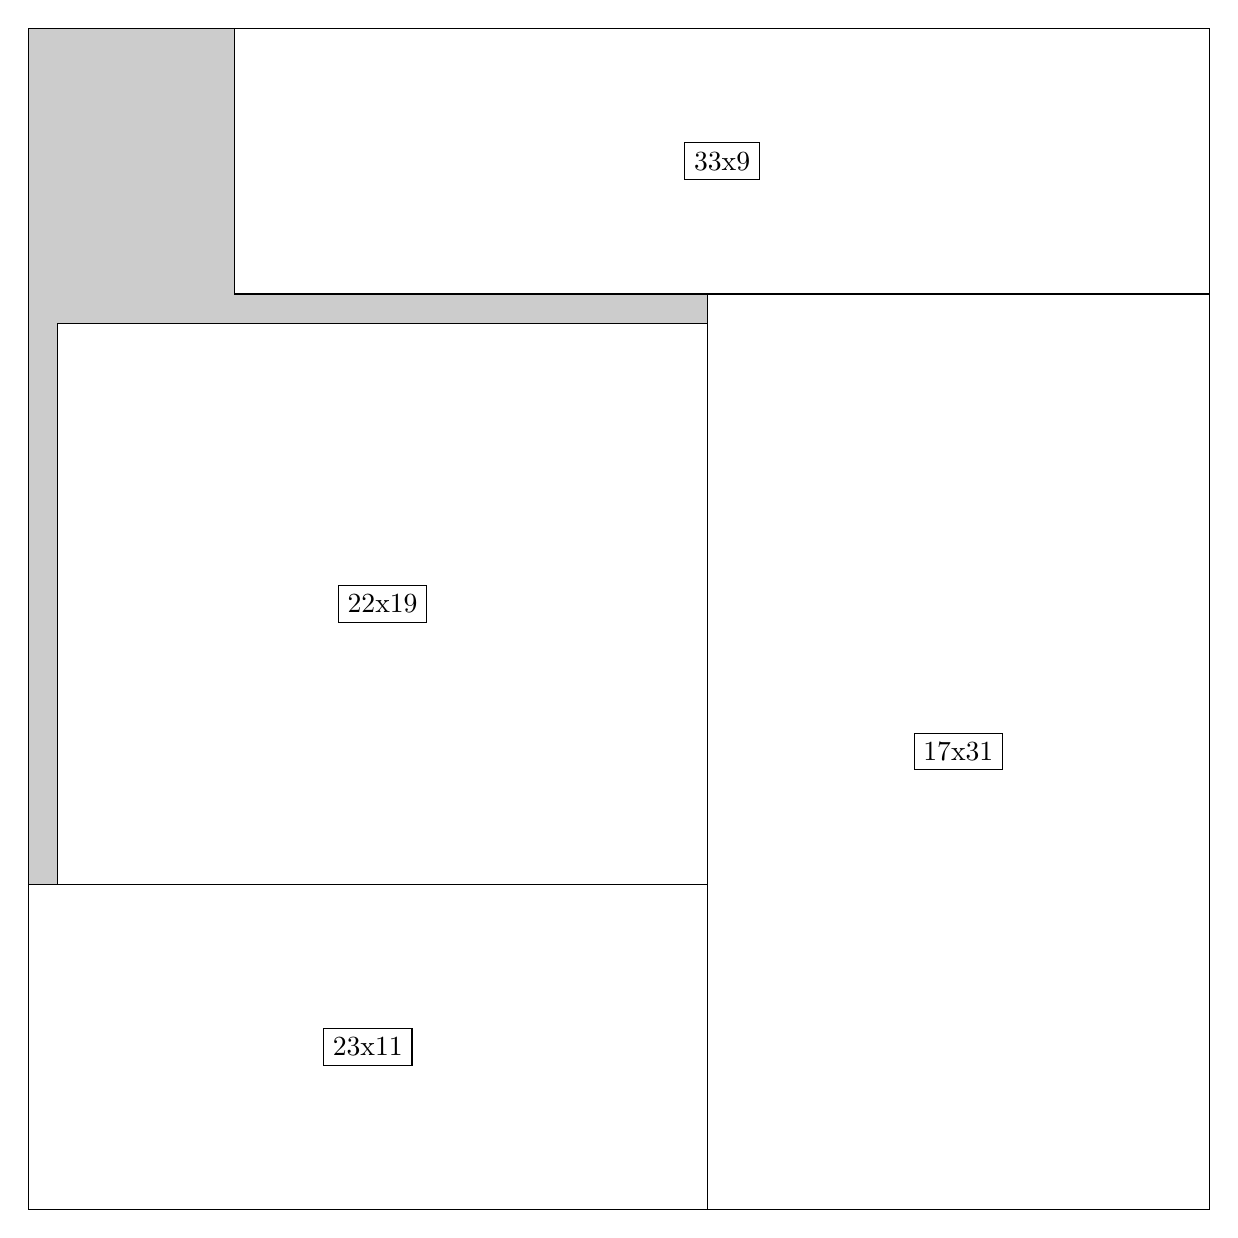
\begin{tikzpicture}[shorten >=1pt,scale=1.0,every node/.style={scale=1.0},->]
\tikzstyle{vertex}=[circle,fill=black!25,minimum size=14pt,inner sep=0pt]
\filldraw[fill=gray!40!white, draw=black] (0,0) rectangle (15.0,15.0);
\foreach \name/\x/\y/\w/\h in {17x31/8.625/0.0/6.375/11.625,23x11/0.0/0.0/8.625/4.125,22x19/0.375/4.125/8.25/7.125,33x9/2.625/11.625/12.375/3.375}
\filldraw[fill=white!40!white, draw=black] (\x,\y) rectangle node[draw] (\name) {\name} ++(\w,\h);
\end{tikzpicture}


w =17 , h =31 , x =23 , y =0 , v =527
\par
w =23 , h =11 , x =0 , y =0 , v =253
\par
w =22 , h =19 , x =1 , y =11 , v =418
\par
w =33 , h =9 , x =7 , y =31 , v =297
\par
\newpage


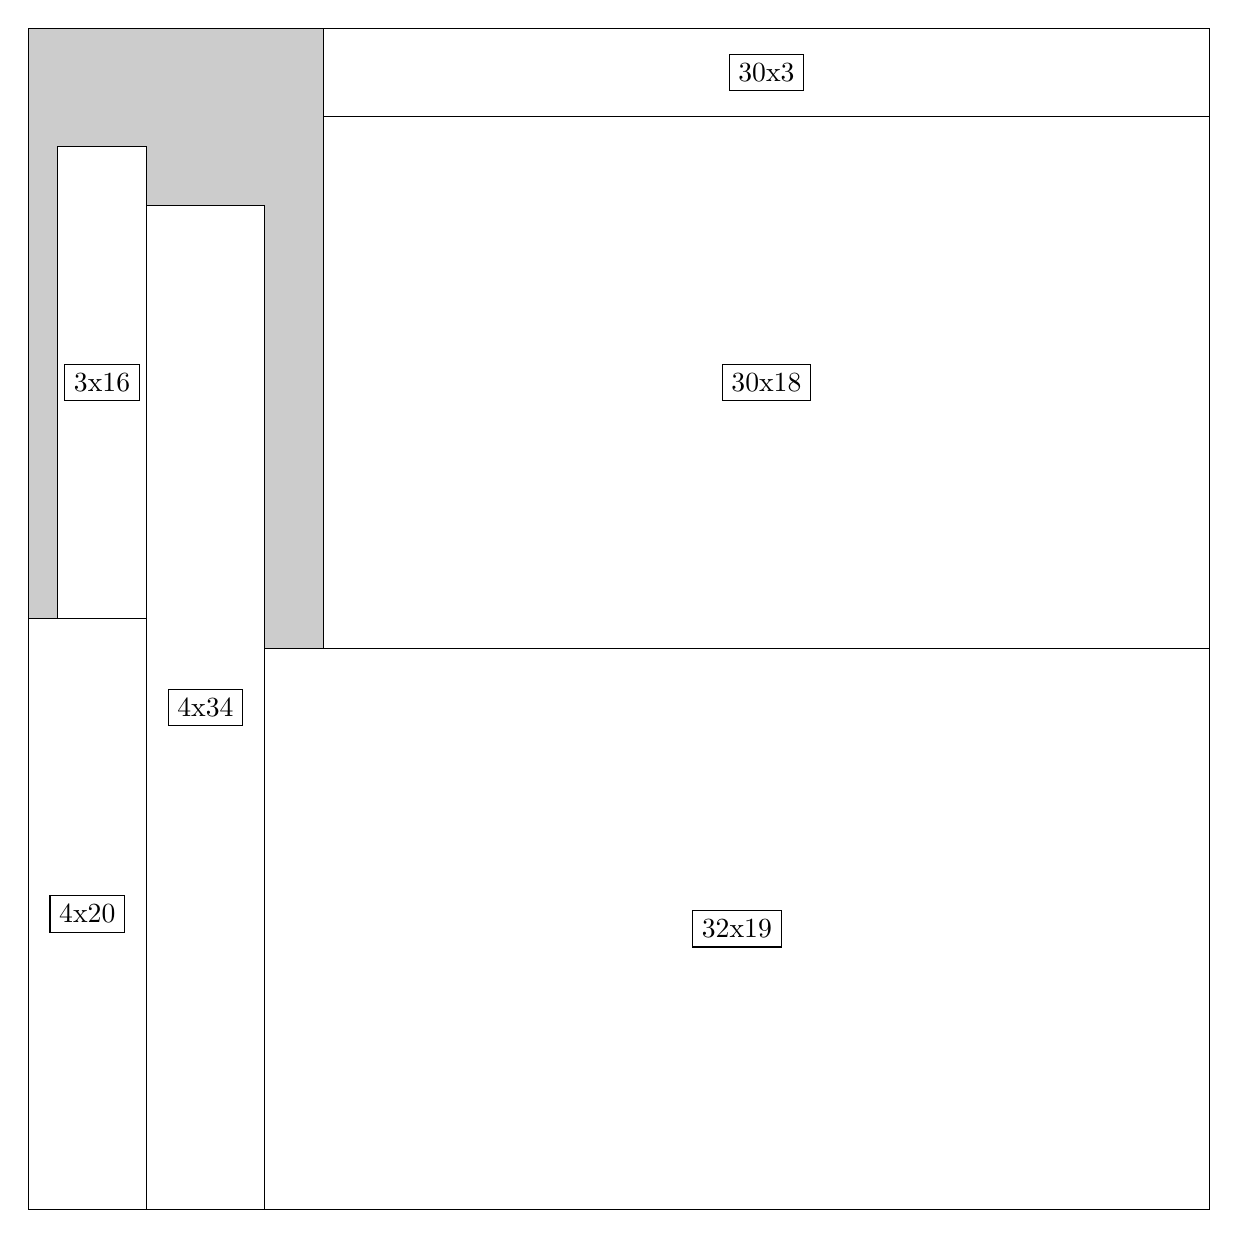
\begin{tikzpicture}[shorten >=1pt,scale=1.0,every node/.style={scale=1.0},->]
\tikzstyle{vertex}=[circle,fill=black!25,minimum size=14pt,inner sep=0pt]
\filldraw[fill=gray!40!white, draw=black] (0,0) rectangle (15.0,15.0);
\foreach \name/\x/\y/\w/\h in {32x19/3.0/0.0/12.0/7.125,30x18/3.75/7.125/11.25/6.75,30x3/3.75/13.875/11.25/1.125,4x34/1.5/0.0/1.5/12.75,4x20/0.0/0.0/1.5/7.5,3x16/0.375/7.5/1.125/6.0}
\filldraw[fill=white!40!white, draw=black] (\x,\y) rectangle node[draw] (\name) {\name} ++(\w,\h);
\end{tikzpicture}


w =32 , h =19 , x =8 , y =0 , v =608
\par
w =30 , h =18 , x =10 , y =19 , v =540
\par
w =30 , h =3 , x =10 , y =37 , v =90
\par
w =4 , h =34 , x =4 , y =0 , v =136
\par
w =4 , h =20 , x =0 , y =0 , v =80
\par
w =3 , h =16 , x =1 , y =20 , v =48
\par
\newpage


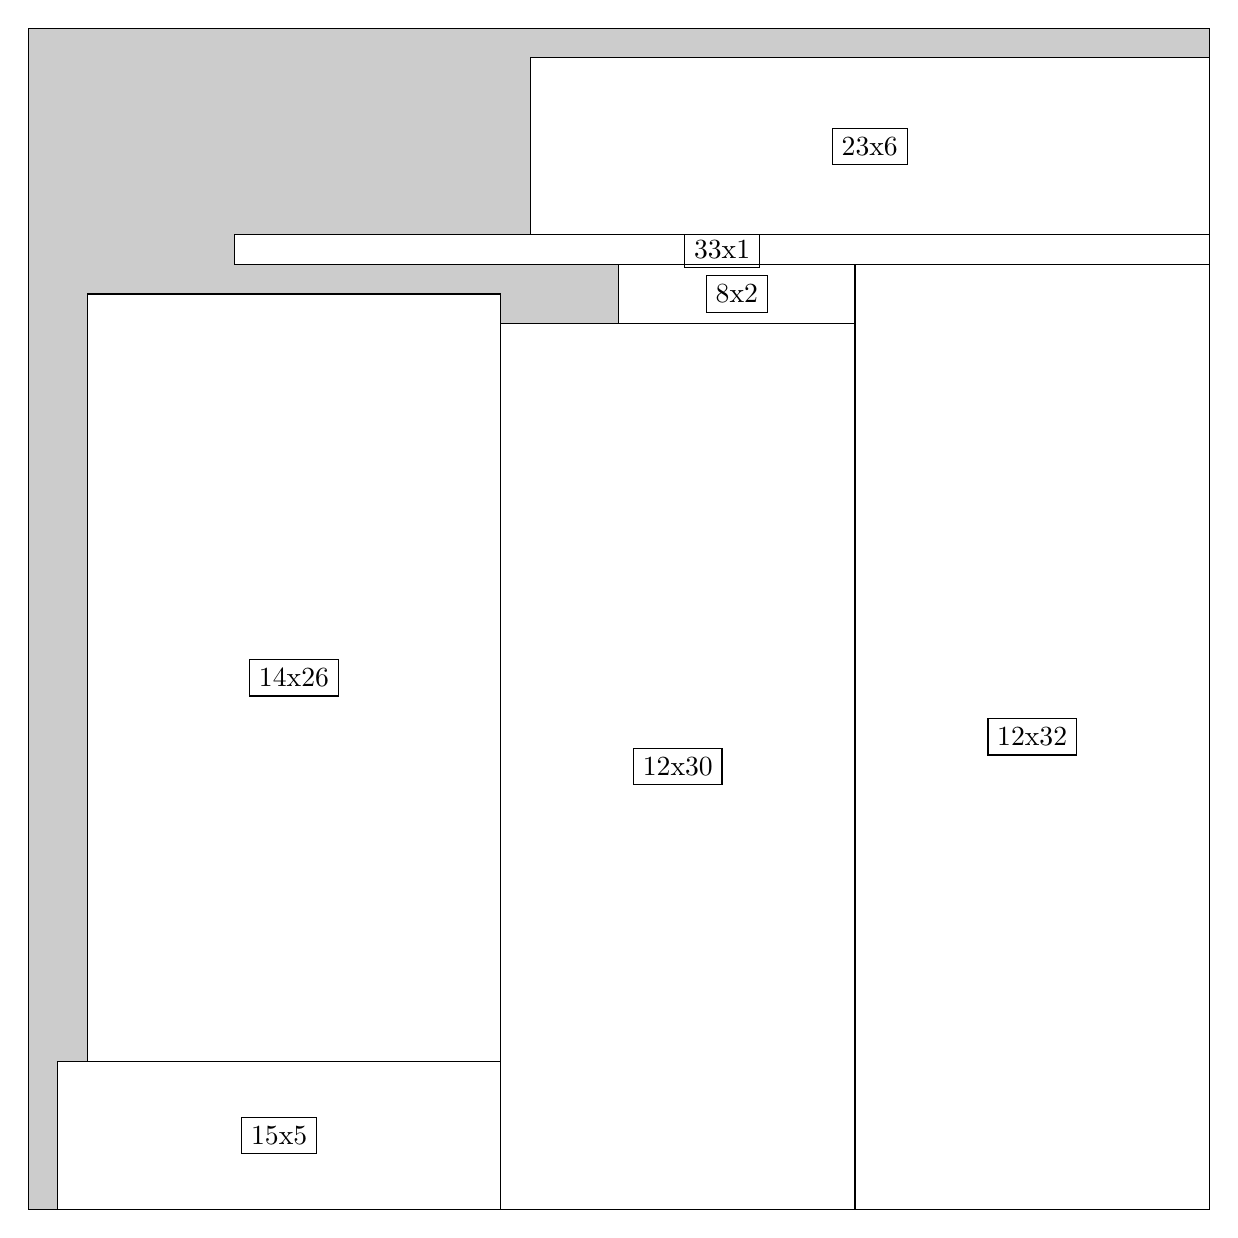
\begin{tikzpicture}[shorten >=1pt,scale=1.0,every node/.style={scale=1.0},->]
\tikzstyle{vertex}=[circle,fill=black!25,minimum size=14pt,inner sep=0pt]
\filldraw[fill=gray!40!white, draw=black] (0,0) rectangle (15.0,15.0);
\foreach \name/\x/\y/\w/\h in {12x32/10.5/0.0/4.5/12.0,12x30/6.0/0.0/4.5/11.25,8x2/7.5/11.25/3.0/0.75,15x5/0.375/0.0/5.625/1.875,14x26/0.75/1.875/5.25/9.75,33x1/2.625/12.0/12.375/0.375,23x6/6.375/12.375/8.625/2.25}
\filldraw[fill=white!40!white, draw=black] (\x,\y) rectangle node[draw] (\name) {\name} ++(\w,\h);
\end{tikzpicture}


w =12 , h =32 , x =28 , y =0 , v =384
\par
w =12 , h =30 , x =16 , y =0 , v =360
\par
w =8 , h =2 , x =20 , y =30 , v =16
\par
w =15 , h =5 , x =1 , y =0 , v =75
\par
w =14 , h =26 , x =2 , y =5 , v =364
\par
w =33 , h =1 , x =7 , y =32 , v =33
\par
w =23 , h =6 , x =17 , y =33 , v =138
\par
\newpage


\end{document}